\section[Software Language Engineering]{\glsdesc{sle}}
\label{sec:back:sle}

As stated by Favre \etal \cite{DBLP:conf/sle/FavreGLP10}, software languages are software.
Like traditional software, they need to be designed, tested, deployed, and maintained.
These activities are grouped under the term \gls{sle} \cite{kleppe2008software}.
Before explaining the role of software languages in this thesis, we will first define them in this section.

\subsection{Software Languages}

\begin{figure}
	\centering
	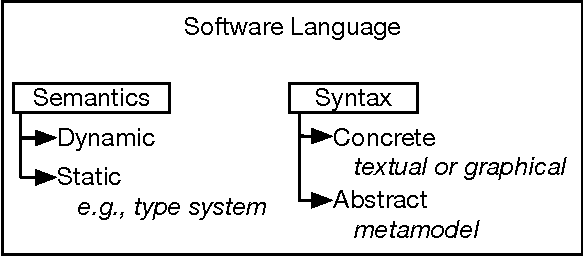
\includegraphics[width=0.5\linewidth]{img/chapt-background/sle/language}
	\caption{Composition of a software language}
	\label{fig:background:sle:lang}
\end{figure}

Most of, not to say all of, developers have used, at least once, a programming language to develop software.
For example, one may use JavaScript to implement client-side behaviour of a web site and another one C to implement a driver.
We can distinguish another kind of language, named modelling languages.
Those models allow developers to implement a model.
For example, we can argue that many developers have already used the HTML language to implement a \gls{dom}\footnote{\textquote{The \gls{dom} is a platform -and language- neutral interface that will allow programs and scripts to dynamically access and update the content, structure and style of [web] documents.}~\cite{DOM:Spec}}
With the emergence of executable models\footnote{Executable models are models that have a semantics attached to their concepts.}, the difference between models and programs are more and more blurry.
So it is for the difference between programming and modelling language.
Hence, Annake Kleppe uses the term \gls{softLge} to combine both kinds of languages.

Another way to classify \glspl{softLge} is by their scope~\cite{DBLP:journals/sigplan/DeursenKV00}.
\Gls{gpl} are languages that can be used for any domain whereas \gls{dsl}\footnote{In this thesis, we do not make the difference between \gls{dsml} and \gls{dsl}} that are restricted to a specific domain.
Using a \gls{gpl}, a developer can use it to implement a full software benefit from great tooling support. 
However, she may manipulate concepts that are different from those of the problem space.
For example, implementing an automatic coffee machine in Java, she will have to manipulate the concept of class, object, functions.
In contrary, \glspl{dsl} are close to their problem domain~\cite{DBLP:journals/smr/DeursenK98} but might suffer from poor tooling support~\cite{voelter2014generic}.
As for \gls{mde}, there are some research efforts to remove this disadvantage~\cite{DBLP:journals/jss/BousseLCWB18}. 
Using \glspl{dsl}, developers can have simpler code, easier to understand and maintain~\cite{DBLP:journals/sigplan/DeursenKV00, DBLP:journals/smr/DeursenK98}.

As depicted in~\Cref{fig:background:sle:lang}, \Glspl{softLge} are composed of two parts~\cite{DBLP:journals/computer/HarelR04}: syntax and semantics.
The syntax defines the element allowed in the language and the semantics their meaning.
We can distinguish two kinds of syntax: the abstract one and the concrete one.
The abstract one defines the different concepts manipulated with the language and their relationships.
A \gls{metamodel} can express it.
The concrete abstract describes how these concepts are represented.
It exists two categories of concrete syntax: graphical and textual.
As for the syntax, there are two kinds of semantics: the static and the dynamic.
The static semantics defines the constraints of the abstract syntax that cannot be directly expressed in the formalism chosen.
For example, the static semantics will define uniqueness constraints for some elements or will forbid any cycle in dependencies (if any).
The type system usually goes in part of the static semantics.
The dynamic semantics defines the behaviour of the language.

When designing a language, engineers can start with the abstract or with the concrete abstract.
In the first case, we say that they define the language in a \gls{model}-first way.
Others will prefer to start by the concrete syntax, and thus they are using a grammar-first approach.
Some tools, like XText~\cite{DBLP:conf/oopsla/EysholdtB10}, can generate the model automatically from the grammar.
 

	
\subsection[SLE in this thesis]{\gls{sle} in this thesis}

In our vision, we argue that uncertainty should be considered as a first-class citizen for modelling frameworks.
This modelling framework should allow the definition of \glspl{metamodel} with uncertainty management capacities.
As described in the previous sections, these \glspl{metamodel} can correspond to the abstract syntax of a language.
As a contribution, we, therefore, propose a language with uncertainty as a first-class citizen: \langName (\cf \Cref{chapt:aintea}).